\section{Introduction}  \label{sec:Introduction}
After observing particle interactions and their corresponding tracks with
bubble or streamer chambers, advances in particle physics required more accurate measurements in order to properly resolve interaction vertices and particle paths \cite{charpak_high-resolution_1984}. The development of detectors with electronic readout and the possibility of stacking and locating tracks at known positions would therefore
prove to be a working and robust solution to this problem. To this end, the advantages of
the gas-flow proportional counters have been known since the 1950s \cite{hendee_gasflow_1956}. They include easy read-out electronic systems, and the possibility to build large detection volumes relying on readily available and afordable gas supplies. Furthermore, operating such detectors at atmospheric pressure reduces the material that charged particles need to traverse from the interaction point, and lowers the requirements for sealing that would otherwise be costly in a vacuum environment.

\begin{figure}[htb!]
  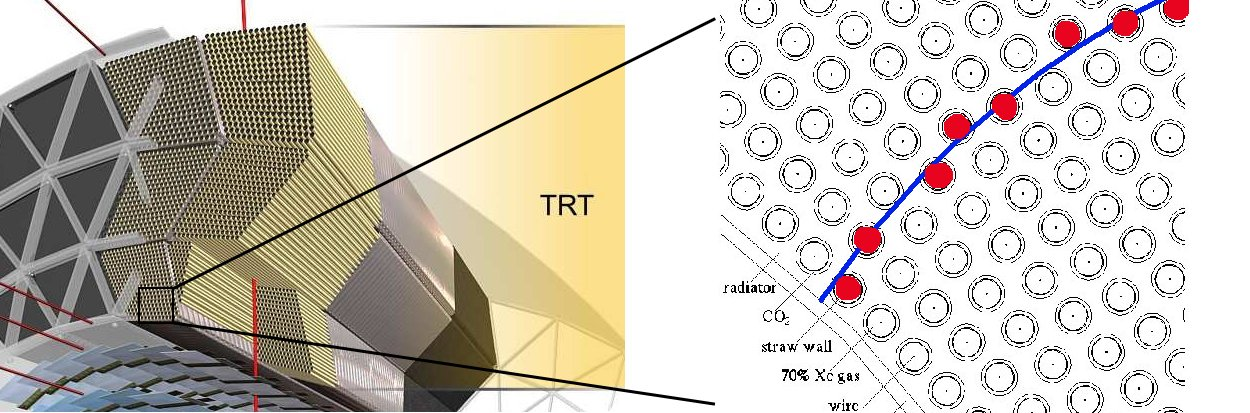
\includegraphics[width=\linewidth]{graphics/ATLAS_TRT_Principle_image}
  \caption{Principle of the ATLAS TRT using proportional counters in a specific
    arrangement. Figure taken from \cite{colliderscope}.}
  \label{fig:colliderscope}
\end{figure}

Gas detectors are often operated in a proportional counting mode, where low charged signals from a particle interaction are amplified in an avalanche that depends, among other things, on the voltage applied and the properties of the gas itself. These porportional chambers are still widely used today \cite{Mindur:2017nqn}. Figure \ref{fig:colliderscope} shows a possible configuration of gas proportional counters within the ATLAS transition radiation tracker, which allows to track the movement of a particle as visualised.

With the versatility of the gas detector comes a variety of challenges, as the choice of gas, tube, wire material, voltage, amplification etc. will each be influencing the resolution and constructability of the detector. In this laboratory, we constructed a proportional counter detector from commercially available parts, calibrated its response when connected to readout electronics, and measured the decay spectra of two radioactive samples: \emph{Iron-55} and \emph{Americium-241}. Our report is organized as follow: Section 2 describes the detector assembly steps and the challenges encoutered during the construction. Section 3 covers the calibration measurements performed to characterize the response of the readout electronics. Details of the energy spectrum calibration are reported in Section 4, while the actual measurements of the spectra contained in the radioactive sources data are presented in Section 5. An analysis of the systematic uncertainties that influence the performance of the gas detector is detailed in Section 6. Finally, a brief overview of measurements made with a more refined gas chamber is included in Section 7.

For the data analysis, CERN's ROOT framework\cite{Brun:1997pa} is used to perform the fit operations through either minimization of LogLikelihood or Chi-squared values.
